\documentclass{standalone}
\usepackage{tikz}
\usetikzlibrary{positioning,fit,calc}
\begin{document}
	
	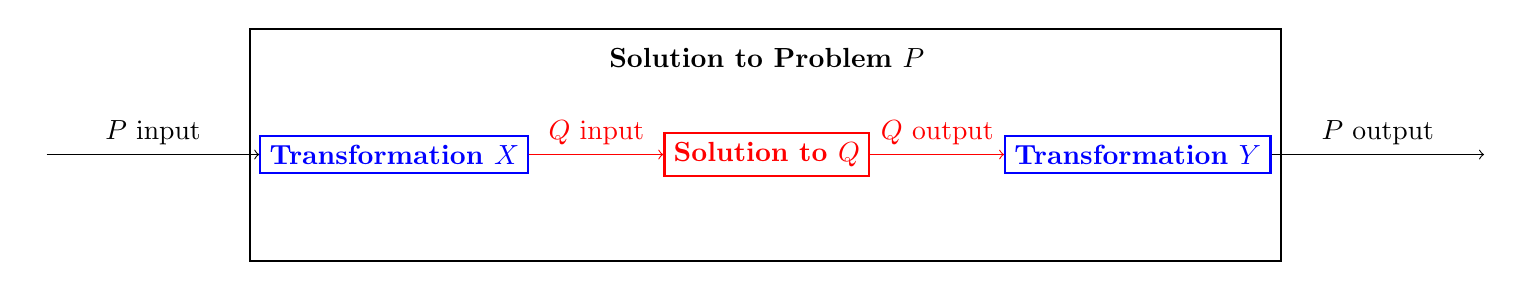
\begin{tikzpicture}[
			node distance=7mm,
			typetag/.style={rectangle, draw=black!50, anchor=north}
	]
	
		\node (titlenode) { \textbf{Solution to Problem $P$}  };
		
		\node (q) [below=of titlenode.south,draw=red,thick,rectangle] { \textcolor{red}{\textbf{Solution to $Q$}} };
		\node (x) [left=of q,thick,draw=blue,rectangle, xshift=-1cm] { \textcolor{blue}{\textbf{Transformation $X$}} };
		\node (y) [right=of q,thick,draw=blue,rectangle, xshift=1cm] { \textcolor{blue}{\textbf{Transformation $Y$}} };
		\node (start) [left=of x, xshift=-2cm] {};
		\node (end) [right=of y, xshift=2cm] {};
		\node (dummy1) [below=of q] {};
		
		\node [draw=black, thick,fit={(titlenode) (q) (x) (y) (dummy1)}] {};
		
		\draw [->,draw=red] (q) -- node[above] {\textcolor{red}{$Q$ output}} (y);
		\draw [->,draw=red] (x) -- node[above] {\textcolor{red}{$Q$ input}} (q);
		\draw [->] (start) -- node[above] {$P$ input} (x);
		\draw [->] (y) -- node[above] {$P$ output} (end);
	\end{tikzpicture}
\end{document}

